\chapter{Related work}
\label{c:relatedwork}

\begin{figure}[b]
	\centering
	
	\begin{subfigure}[b]{0.45\textwidth}
		\centering
        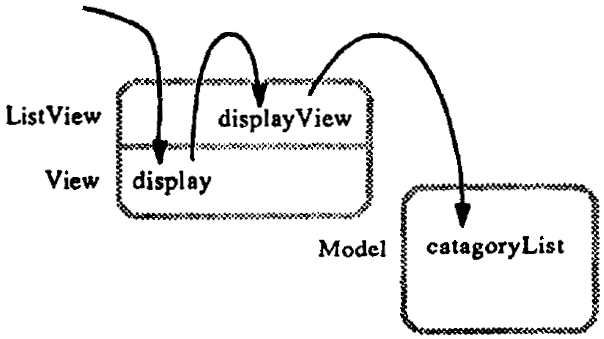
\includegraphics[width=\textwidth]{../images/06-Cunningham-Diagram}
        \caption[Foo]{}
		\label{fig:06-1-Cunningham}
	\end{subfigure}
	\quad
	\begin{subfigure}[b]{0.45\textwidth}
		\centering
		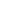
\includegraphics[width=\textwidth,height=2cm]{../images/foo}
		\caption[Bar]{}
		\label{fig:06-1}
	\end{subfigure}
	
	\caption[TOC Caption]{
		a) Cunningham's and Beck's notion of diagramming object interactions, taken from \cite{cunningham_diagram_1986}.
		b) ...
	}
	\label{fig:06-1}
\end{figure}

Cunningham and Beck propose a syntax for diagramming the message sending dialogue between objects in object-oriented computations (see Figure \ref{fig:06-1-Cunningham}) and extend the Smalltalk-80 debugger to allow for the automatic generation of such diagrams \cite{cunningham_diagram_1986}.
Similar to \textsc{PathObjects}, objects are drawn as boxes and message sends are represented by directed arcs between them.
Unlike the notation used by \textsc{PathObjects}, the space inside the boxes is not used to model the object state, but to emphasize method overrides and calls to implementations of superclasses.
Therefore, the class hierarchy is represented by layers in a box.
Since the authors regard overriding as the more important concept over inheritance, subclasses are placed above superclasses in these layers.

Systä et al. present a reverse engineering environment called \textsc{Shimba} \cite{systa_shimba_2001}, which supports both static and dynamic analysis of Java software systems.
Static information about software entities like classes, interfaces and their relationships is extracted from the bytecode representation and visualized using \textsc{Rigi} \cite{muller_understanding_1993} in the form of directed dependency graphs.
Besides the computation of some of the metrics of Chidamber's and Kemerer's suite \cite{chidamber_metrics_1994}, \textsc{Rigi} also can be utilized to build abstractions, for instance by aggregating classes into their respective packages.
Runtime traces are collected with the help of a customized SDK debugger and can be synthesized as UML-like sequence and statechart diagrams through \textsc{SCED} \cite{koskimies_automated_1998,systa_understanding_2000}.
\textsc{Shimba} supports bidirectional model slicing between \textsc{Rigi} graphs and \textsc{SCED} diagrams.
On one side, \textsc{Rigi} can be used to restrict the amount of collected execution events through the selection of components of interest. Thus, the scope of the generated \textsc{SCED} diagrams is reduced.
On the other side, starting from a \textsc{SCED} diagram, static views covering the affected components can be obtained.